%%%%%%%%%%%%  math symb %%%%%%%

\newcommand{\ba}{\mathbf{a}}
\newcommand{\bc}{\mathbf{c}}
\newcommand{\bA}{\mathbf{A}}
\newcommand{\bB}{\mathbf{B}}
\newcommand{\bb}{\mathbf{b}}
\newcommand{\bO}{\mathbf{0}}% null vector
\newcommand{\bD}{\mathbf{D}}

\newcommand{\bG}{\mathbf{G}}
\newcommand{\be}{\mathbf{e}}
\newcommand{\bE}{\mathbf{E}}
\newcommand{\bF}{\mathbf{F}}
\newcommand{\bH}{\mathbf{H}}
\newcommand{\bh}{\mathbf{h}}
\newcommand{\br}{\mathbf{r}}
\newcommand{\bR}{\mathbf{R}}

\newcommand{\bp}{\mathbf{p}}
\newcommand{\bs}{\mathbf{s}}
\newcommand{\bI}{\mathbf{I}} 
\newcommand{\bK}{\mathbf{K}}

\newcommand{\bl}{\mathbf{l}}
\newcommand{\bM}{\mathbf{M}}
\newcommand{\bS}{\mathbf{S}}

\newcommand{\bt}{\mathbf{t}}
\newcommand{\bg}{\mathbf{g}}
\newcommand{\bT}{\mathbf{T}}
\newcommand{\bu}{\mathbf{u}}
\newcommand{\bv}{\mathbf{v}}
\newcommand{\bV}{\mathbf{V}}

\newcommand{\bw}{\mathbf{w}}
\newcommand{\bW}{\mathbf{W}}
\newcommand{\bx}{\mathbf{x}}
\newcommand{\bX}{\mathbf{X}}
\newcommand{\by}{\mathbf{y}}
\newcommand{\bY}{\mathbf{Y}}
\newcommand{\bz}{\mathbf{z}}
\newcommand{\bZ}{\mathbf{Z}}
\newcommand{\bP}{\mathbf{P}}
%
%

\newcommand{\bsA}{\boldsymbol{A}}
\newcommand{\bsB}{\boldsymbol{B}}

\newcommand{\bsd}{\boldsymbol{d}}
%\newcommand{\bsI}{\boldsymbol{I}}
\newcommand{\bse}{\boldsymbol{e}}
\newcommand{\bsE}{\boldsymbol{E}}

\newcommand{\bsn}{\boldsymbol{n}}
\newcommand{\bsg}{\boldsymbol{g}}

\newcommand{\bsr}{\boldsymbol{r}}
\newcommand{\bss}{\boldsymbol{s}}
\newcommand{\bsS}{\boldsymbol{S}}
\newcommand{\bst}{\boldsymbol{t}}
\newcommand{\bsT}{\boldsymbol{T}}
\newcommand{\bsv}{\boldsymbol{v}}
\newcommand{\bsw}{\boldsymbol{w}}
\newcommand{\bsW}{\boldsymbol{W}}
\newcommand{\bsx}{\boldsymbol{x}}
\newcommand{\bsX}{\boldsymbol{X}}
\newcommand{\bsy}{\boldsymbol{y}}
\newcommand{\bsY}{\boldsymbol{Y}}
\newcommand{\bsz}{\boldsymbol{z}}
\newcommand{\bsZ}{\boldsymbol{Z}}
\newcommand{\bsH}{\boldsymbol{H}}

% caligraphic
\newcommand{\cN}{\mathcal{N}}
\newcommand{\cM}{\mathcal{M}}
\newcommand{\cI}{\mathcal{I}}
\newcommand{\cW}{\mathcal{W}}
\newcommand{\cL}{\mathcal{L}}
\newcommand{\cR}{\mathcal{R}}
\newcommand{\cX}{\mathcal{X}}
\newcommand{\cY}{\mathcal{Y}}
\newcommand{\cZ}{\mathcal{Z}}
\newcommand{\cT}{\mathcal{T}}
\newcommand{\cB}{\mathcal{B}}
\newcommand{\cD}{\mathcal{D}}

\newcommand{\cJ}{\mathcal{J}}
\newcommand{\cG}{\mathcal{G}}
\newcommand{\cH}{\mathcal{H}}
\newcommand{\cK}{\mathcal{K}}

\newcommand{\cO}{\mathcal{O}}



%
\newcommand{\diff}{\mathrm{d}}
%
%
% grec
\newcommand{\bspi}{\boldsymbol{\pi}}
\newcommand{\bsmu}{\boldsymbol{\mu}}
\newcommand{\bsnu}{\boldsymbol{\nu}}
\newcommand{\bsalpha}{\boldsymbol{\alpha}}
\newcommand{\bsbeta}{\boldsymbol{\beta}}
\newcommand{\bsgamma}{\boldsymbol{\gamma}}
\newcommand{\bsGamma}{\boldsymbol{\Gamma}}
\newcommand{\bsomega}{\boldsymbol{\omega}}
\newcommand{\bsOmega}{\boldsymbol{\Omega}}
\newcommand{\bsSigma}{\boldsymbol{\Sigma}}
\newcommand{\bssigma}{\boldsymbol{\sigma}}
\newcommand{\bslambda}{\boldsymbol{\lambda}}
\newcommand{\bsLambda}{\boldsymbol{\Lambda}}
\newcommand{\bstheta}{\boldsymbol{\theta}}
\newcommand{\bsTheta}{\boldsymbol{\Theta}}
\newcommand{\bseta}{\boldsymbol{\eta}}
\newcommand{\bsepsilon}{\boldsymbol{\epsilon}}
\newcommand{\bspsi}{\boldsymbol{\psi}}
\newcommand{\bsPsi}{\boldsymbol{\Psi}}
\newcommand{\bsvPsi}{\boldsymbol{\varPsi}}
\newcommand{\bsPhi}{\boldsymbol{\Phi}}
\newcommand{\bsphi}{\boldsymbol{\varphi}}%%----
\newcommand{\bstau}{\boldsymbol{\tau}}
\newcommand{\bszeta}{\boldsymbol{\zeta}}
\newcommand{\bsxi}{\boldsymbol{\xi}}

\newcommand{\bPi}{\mathbf{\Pi}}

%\newcommand{\R}{\mathds{R}}
\newcommand{\Indicatrice}{\mathds{1}}

\newcommand{\Identity}{\textbf{I}}

%%---------------------%%

\newcommand{\tp}{\widetilde{p}}
\newcommand{\ts}{\widetilde{\boldsymbol{s}}}
\newcommand{\tT}{\widetilde{\textbf{T}}}
%
%
\newcommand{\E}{\mathbb{E}}
\newcommand{\V}{\mathbb{V}}
\newcommand{\Pro}{\mathbb{P}}
\newcommand{\R}{\mathbb{R}}
\newcommand{\Nset}{\mathbb{N}}	

\newcommand{\N}{\mathbb{N}}
\newcommand{\M}{\mathbb{M}}

\newcommand{\ocap}{\textcircled{\scriptsize{$\cap$}}}
\newcommand{\ocup}{\textcircled{\scriptsize{$\cup$}}}
\newcommand{\Bocup}{\textcircled{\Big{$\cup$}}}
\newcommand{\Bocap}{\huge\textcircled{\LARGE$\cap$}}
%\newcommand{\oplus}{\textcircled{\scriptsize{$+$}}}
\newcommand{\decond}{\rotatebox{90}{$\multimap$}}
\newcommand{\tdef}{\stackrel{\textrm{\tiny{$\triangle$}}}{=}}
\newcommand{\iid}{i.i.d.}
\newcommand{\cf}{\textit{c.f.}}
\newcommand{\pa}{par}
\newcommand{\kernel}{\kappa}
\newcommand{\pen}{\Gamma}
\newcommand{\inde}{\perp\!\!\!\perp}
\newcommand{\grad}{\bigtriangledown}
\newcommand{\hadaprod}{\bullet}
\newcommand{\tr}{\mathrm{tr}}
%%
\newcommand{\BIC}{\text{BIC}}
\newcommand{\AIC}{\text{AIC}}
\newcommand{\ICL}{\text{ICL}}
\newcommand{\NEC}{\text{NEC}}

 


\documentclass[12pt]{article}
\usepackage[utf8]{inputenc}
\usepackage[T1]{fontenc}
\usepackage[francais]{babel}

\setlength{\oddsidemargin}{0in}  %left margin position, reference is one inch
\setlength{\textwidth}{6.5in}    %width of text=8.5-1in-1in for margin
\setlength{\topmargin}{-0.5in}    %reference is at 1.5in, -.5in gives a start of about 1in from top
\setlength{\textheight}{9in}     %length of text=11in-1in-1in (top and bot. marg.) 

\usepackage{amsmath,amssymb}
\usepackage{amsthm}
\usepackage{graphicx}% Include figure files
\usepackage{caption}
\usepackage{xcolor}% Include colors for document elements
\usepackage{dcolumn}% Align table columns on decimal point
\usepackage{bm}% bold math
\usepackage{float}
%\usepackage[nolists, nomarkers, figuresfirst]{endfloat}
\usepackage{url}
\usepackage[francais]{babel}
\usepackage{lmodern}
\usepackage{mathrsfs}
\DeclareSymbolFontAlphabet{\mathcal}   {symbols}
\DeclareMathAlphabet{\mathcal}{OMS}{Zplm}{m}{n}
\SetMathAlphabet{\mathcal}{bold}{OMS}{zplm}{b}{n}
 
%\usepackage[authoryear,round]{natbib}
%\usepackage[authoryear, round]{natbib}
%\usepackage[super,comma]{natbib}

%\usepackage[superscript,biblabel]{cite}
%\usepackage[authoryear, round]{natbib}
 \usepackage[
%                 pdfpagelayout = useoutlines,
%                 bookmarks,
%                 bookmarksopen = true,
%                 bookmarksnumbered = true,
                  breaklinks = true,
%                 linktocpage,
%                 pagebackref,
                 colorlinks = true,
                 linkcolor = red,
                 urlcolor  = black, %green,
                 citecolor = blue,
                 anchorcolor = green,
%%                 hyperindex = true,
%%                 hyperfigures
                 ]{hyperref} 
 


%\input{mymathsym.tex}


\title{Utilisation de la programmation dynamique pour la segmentation de series temporelles} 
\smallbreak
\author{Aline Canard\thanks{Master2 SAAD, Université de Caen Normandie}}
\smallbreak
%\date{}
\smallbreak
\begin{document}
\maketitle


\begin{center}


\hfill \break
\thanks
\smallbreak
\medbreak

\subsubsection*{Abstract}
\end{center}
De nombreux domaines scientifiques et techniques ont besoin de représenter des paramètres qui évoluent au cours du temps et de les modéliser. Il s'agit de pouvoir en extraire différentes séquences de fonctionnement et pour chacun des régimes définis y proposer un modèle de régression. Ce document présente les résultats d'une segmentation par programmation dynamique et propose de modéliser chaque régime par une régression polynomiale.


 
\clearpage


\renewcommand{\baselinestretch}{1.5}
\normalsize

\section{Introduction}
\label{sec:Introduction}
Les séries temporelles interviennent dans de nombreux domaines tels que la finance, l'économie, ingénierie, la bioinformatique pour représenter les variations d'une mesure au cours du temps. Le domaine d'étude de ce type de données se nomme "analyse fonctionnelle" \cite{RamsayAndSilvermanFDA2005,ramsayandsilvermanAppliedFDA2002,FerratyANDVieuBook}. La philosophie repose sur l'idée de ne pas traiter les données comme des observations stockées dans un vecteur mais comme des valeurs (discrètes) d'une fonction. Les individus sont donc considérés non pas comme des vecteurs  mais comme des fonctions. Des techniques de modélisation vont permettre de donner une représentation synthétique de tels phénomènes. Ce document présentera une de ces méthodes de segmentation de série temporelle : la régression par morceaux basée sur un modèle polynomial hétéroscédastique \cite{chamroukhi_et_al_NN2009,Chamroukhi-IJCNN-2009,Chamroukhi-FDA-2018}. La méthode utilisée est la programmation dynamique. Les paramètres du modèle seront estimés par maximum de vraisemblance. En général, cette méthode est plutôt utilisée dans le cas de changement abruptes de régimes.
\smallbreak

\begin{figure}[H] 
\centering
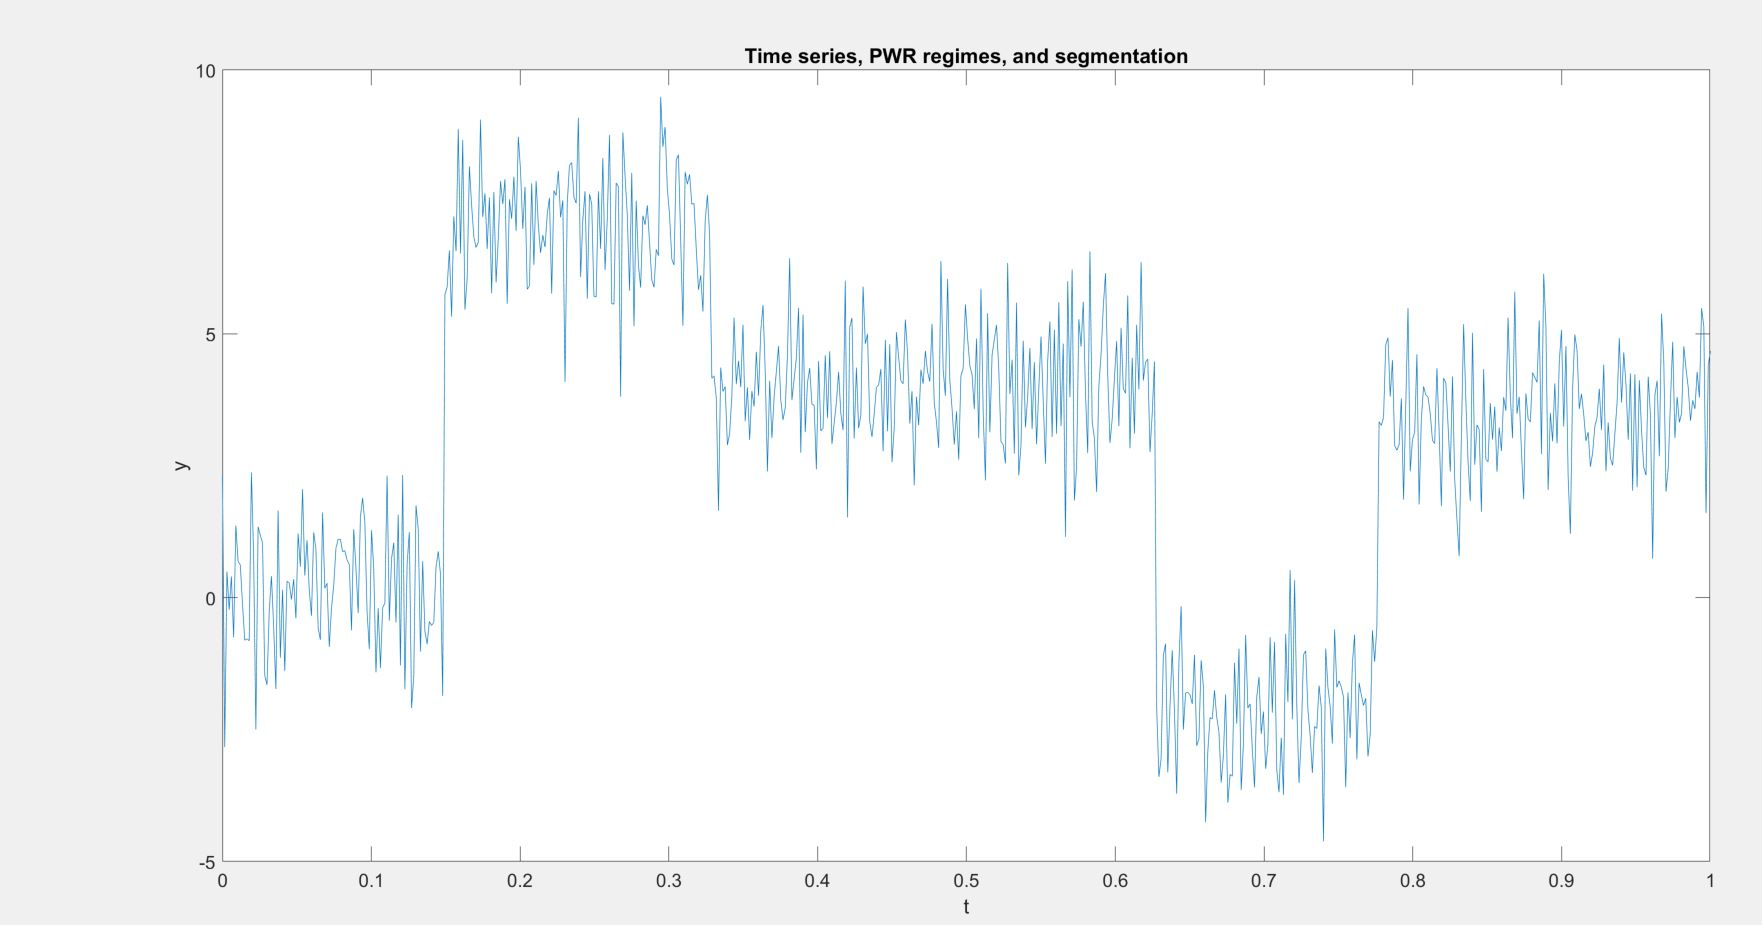
\includegraphics[scale=.5]{serietempinit.jpg}
\caption{\label{fig: switch curve example} Exemple de série temporelle à segmenter}
\end{figure} 
%
%%%%%%%%%%%%%%%%%%%%%%%%%%%%%%%%%%%%%%%%%%%%%%%%%%%%%%%%
% End of figures part for introduction
%%%%%%%%%%%%%%%%%%%%%%%%%%%%%%%%%%%%%%%%%%%%%%%%%%%%%%%%

Ce document a pour but de présenter la méthode mathématique et le code R réalisé pour effectuer la segmentation de telle série temporelle. Il est basé sur la publication:  \cite{RamsayAndSilvermanFDA2005,ramsayandsilvermanAppliedFDA2002,FerratyANDVieuBook}. 

Dans une première partie, le modèle sera spécifié, et cela permettra de justifier le choix de la programmation dynamique comme méthode de segmentation. La deuxième partie s'attachera à expliquer les différentes fonction du code R et leur organisation. Enfin les représentation graphiques de la segmentation réalisée avec l'algorithme R sur un exemple de série temporelle seront présentées en fin de document.


\section{Modèle de mélange pour des données fonctionnelles}
\label{sec: FMM formulation for FDA}


\subsection{Définition du modèle}
\label{ssec: def1}
\smallbreak

Soit ${\bx}= ({\mathcal{X}}_{1},...,{\mathcal{X}}_{n})$, une observation d'une série temporelle où les $x_{i}$ sont observés au temps $t_{i}$. Le modèle de régression polynomiale par morceaux suppose que la série temporelle soit composée de $K$ régimes sur $K$ intervalles dont les indices de bornes peuvent être notés : $\bsgamma=(\gamma_{1},...,\gamma_{K+1})$ avec $\gamma_{1}=0$ et $\gamma_{K+1}=n$. Cela définit une partition de la série temporelle en $K$ segments polynomiaux $({\bx}_{1},...,{\bx}_{K})$, de longueur $n_{1},...,n_{K}$ où ${\bx}_{K}=\{{\bx}_{i}| i\in I_{K}\}$ est l'ensemble des éléments d'un segment $k$ dont les indices sont : $I_{K}=(\bsgamma_{K},\bsgamma_{K+1}]$. Les modèles standards de régression polynomiale sont des modèles homoscédastiques puisqu'ils supposent que les différents modèles de régression polynomiale ont la même de bruit. Dans notre cas, nous considérons le cadre plus général d'un modèle hétéroscédastique; ce qui permet d'avoir une variance de bruit entre les différents modèles de régression polynomiale.On peut le définir ainsi : 
\begin{equation}
\forall{i}=1,..n, {\bx}_{i}=\bsbeta^{T}_{k}\br_{i} + \sigma_{k}\epsilon_{i}; \epsilon_{i}\sim \cN (0,1),
\label{eq:Hyp1}
\end{equation}
où $k$ est tel que $i\in I_{k}, \bsbeta_{k}$ est le vecteur des coefficients de la $(p+1)^{eme}$ dimension d'un polynôme de degré $p$ associé au $k^{eme}$ segment, avec $k\in \{1,..,K\}$, 
$\br_{i}=(1,t_{i},t_{i}^{2},...,t_{i}^{p})^T$ est le vecteur de monômes de dimension $(p+1)$ associé au paramètre $\bsbeta_{k}$, et les $\epsilon_{i}$ sont des variables aléatoires, indépendantes et distribuées selon une loi normale. Elles représentent un bruit additionnel dans chaque segment k.  

\begin{figure}[H] 
\centering
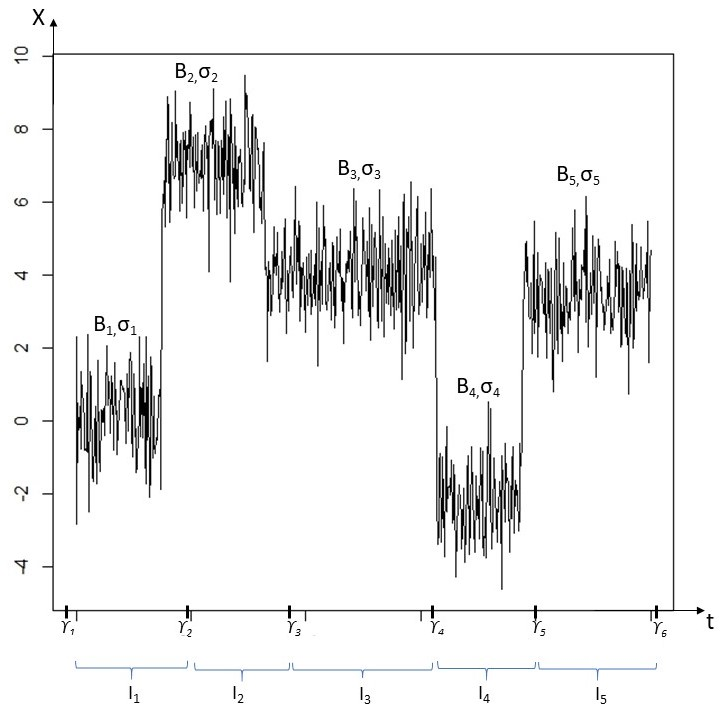
\includegraphics[scale=.5]{SchemaSerieTemp.JPG}
\caption{\label{fig: tempseries2} Série temporelle avec les notations}
\end{figure} 
%
%%%%%%%%%%%%%%%%%%%%%%%%%%%%%%%%%%%%%%%%%%%%%%%%%%%%%%%%
% End of figures part for introduction
%%%%%%%%%%%%%%%%%%%%%%%%%%%%%%%%%%%%%%%%%%%%%%%%%%%%%%%%
L'objectif de la segmentation sera de positionner les $\bsgamma_{k}$ de façon optimale.\\


A l'instant $t$, on peut écrire:
${\bx}_{t}=$
 $\left \{
   \begin{array}{l}
     \bsbeta_{1}^T \br_{t} + \sigma_{1}\epsilon_{t}, \, si\  {\bx}_{t}\in I_{1}\\
     \bsbeta_{2}^T \br_{t} + \sigma_{2}\epsilon_{t}, \, si\  {\bx}_{t}\in I_{2} \qquad \textrm{où}\ \epsilon_{t}\ \sim \mathcal{N}(0,1)\, \\
     ...\\
     \bsbeta_{K}^T \br_{t} + \sigma_{K}\epsilon_{t}, \, si\  {\bx}_{t}\in I_{K}\\
       \end{array}
   \right. $
\smallbreak
\subsection{Estimation des paramètres du modèle par maximum de vraisemblance}
\label{ssec: 2-2}
\smallbreak
Avec ce modèle, les paramètres peuvent s'écrire de la forme : $(\bspsi,\bsgamma)$ où  $\bspsi=(\bsbeta_{1},...,\bsbeta_{k},\bssigma^2_{1},..,\bssigma^2_{k})$ est l"ensemble des coefficients polynomiaux et des variances de bruit, et $\bsgamma=(\gamma_{1},...,\gamma_{K+1})$ l'ensemble des points de rupture. L'estimation des paramètres se fera par maximum de vraisemblance. L'indépendance conditionnelle des données est supposée. Ainsi, d'après le modèle défini dans l'équation  (Equation\ref{eq:Hyp1}), on peut montrer que dans chaque segment $k$, ${\bx}_{i}$ a une distribution gaussienne de moyenne $\bsbeta^{T}_{k}\br_{i}$ et de variance $\sigma^2_{k}$ et, par conséquent, que la log-vraisemblance du vecteur paramètre $(\bspsi,\bsgamma)$ caractérisant le modèle de régression polynomiale par morceaux est la somme des log-vraisemblances locales sur les $K$ segments comme suit :
\begin{equation}
\begin{split}
 L(\bspsi,\bsgamma,{\bx}) & = \prod_{k=1}^{K}p({\bx}_{k},\bspsi,\bsgamma,{\bx}) \\
\ln(L(\bspsi,\bsgamma,{\bx})) & = \sum_{k=1}^{K} ln(p({\bx}_{k},\bspsi,\bsgamma,{\bx})) \\
&                  = \sum_{k=1}^{K} ln( \prod_{t=\gamma_{K}+1}^{\gamma_{K+1}}   \mathcal{N}({\bx}_{t},\bsbeta^{T}_{k}\br_{i},\sigma^2_{k}))\\
&       			 = \sum_{k=1}^{K} ln( \prod_{t \in I_k}   \mathcal{N}({\bx}_{t},\bsbeta^{T}_{k}\br_{i},\sigma^2_{k}))\\
&       			 = \sum_{k=1}^{K} \sum_{t \in I_k}  ln(  \mathcal{N}({\bx}_{t},\bsbeta^{T}_{k}\br_{i},\sigma^2_{k}))\\
&       			 = \sum_{k=1}^{K} \sum_{t \in I_k}  ((-\frac{1}{2}))(\frac{{\bx}_{t}-\bsbeta^{T}_{k}\br_{i}}{\sigma_{k}})^2 + \ln (\sigma^2_{k}))+Constante\\
\label{eq:Hyp2}
\end{split}
\end{equation}

Maximiser la log-vraisemblance revient à minimiser le critère ci-dessous selon les paramètres $\bspsi$ et $\bsgamma$:

\begin{equation}
J(\bspsi,\bsgamma) =  \sum_{k=1}^{K} \Big[ \frac{1}{\sigma^2_{k}} \sum_{t \in I_k} ({\bx}_{t}-\bsbeta^{T}_{k}\br_{i})^2 + n_{k}\ln (\sigma^2_{k}) \Big]
\label{eq:Hyp3}
\end{equation}  
où $n_{k}$ est le nombre d'éléments dans le segment $k$.\\
Vue la forme de cette log-vraisemblance (en log de somme), il n'est pas possible de trouver une solution analytique. Par contre, comme le critère $J$ est additif sur les $K$ segments, on peut utiliser l'algorithme de Fisher (Fisher, 1958; Lechevallier, 1990), procédé de programmation dynamique (Bellman, 1961 ; Brailovsky et Kempner, 1992) pour réaliser la minimisation globale. Ce procédé dynamique a une complexité en temps en $O(Kp^2n^2)$; ce qui peut être coûteux en temps machine dans le cadre de jeux de données volumineux. 

\smallbreak
\subsection{Approximation et segmentation d'une série temporelle par la méthode de régression par morceaux}
\label{ssec: 2-3}
\smallbreak
Une fois les paramètres estimés, la segmentation d'une série temporelle, qui peut être représentée par le vecteur des classes :  
$\widehat{\bz}=( \widehat{z}_1,...,\widehat{z}_n)$, où $\widehat{z}_i \in \{1,..K\}$, peut être déduit en posant $\widehat{z}_i = k$ si $i \in (\widehat{\bsgamma}_{K},\widehat{\bsgamma}_{K+1}]$; les paramètres  $(\widehat{\bspsi},\widehat{\bsgamma})$ ayant été obtenus par le procédé de programmation dynamique.
Puis une approximation de la série temporelle est donnée par $\widehat{{\bx}}_{i}=\sum_{k=1}^{K} \widehat{z}_{ik}\widehat{\bsbeta}^{T}_{k}\br_{i}$ où $\widehat{z}_{ik}=1$ si $\widehat{z}_{i}=k$ et $\widehat{z}_{ik}=0$ sinon. La formulation vectorielle de la série temporelle approchée $\widehat{{\bx}}$ peut s'écrire: 
\begin{equation}
\widehat{{\bx}}=\sum_{k=1}^{K} \widehat{\bz}_{k}\widehat{\bsbeta}_{k}
\label{eq:Hyp4}
\end{equation}  
où $ \widehat{\bz}_{k}$ est une matrice diagonale dont les éléments diagonaux sont $( \widehat{z}_1,...,\widehat{z}_n)$ et 
$$
\bT=\begin{pmatrix}
   1 & \bt_{1} & \bt^2_{1} & \cdots & \bt^p_{1} \\
   1 & \bt_{2} & \bt^2_{2} & \cdots & \bt^p_{2}  \\
   \vdots & \vdots &\vdots &\vdots\\
   1 & \bt_{n} & \bt^2_{n} & \cdots & \bt^p_{n}  
\end{pmatrix}
$$
est la matrice de régression de dimension $[n\times(p+1)]$.

\section{Description de l'algorithmique de segmentation}
\smallbreak
Le programme complet de segmentation d'une série temporelle selon le modèle de régression polynomiale par morceaux par la méthode de programmation dynamique a été implémenté en R. La programmation dynamique Le principe de cette méthode consiste à décomposer le problème en sous-problèmes et à établir une relation de récurrence avec les solutions optimales des sous-problème. L'algorithme proposé par Lechevalier en 1990 est basé sur l'approche de Fisher. Le principe est de maximiser dans ce cas la somme des log-vraisemblances des K sous-modèles de régression relatifs aux K classes ou intervalles, qui est un critère additif sur les K intervalles. 
Le programme en R contient 6 sous-fonction. La manière dont ces fonctions s'imbriquent est présentée via la carte mentale ci-dessous :
\smallbreak
\subsection{Carte mentale de l'ensemble du programme}
\label{ssec: CM}
\smallbreak
\begin{figure}[H] 
%\centering
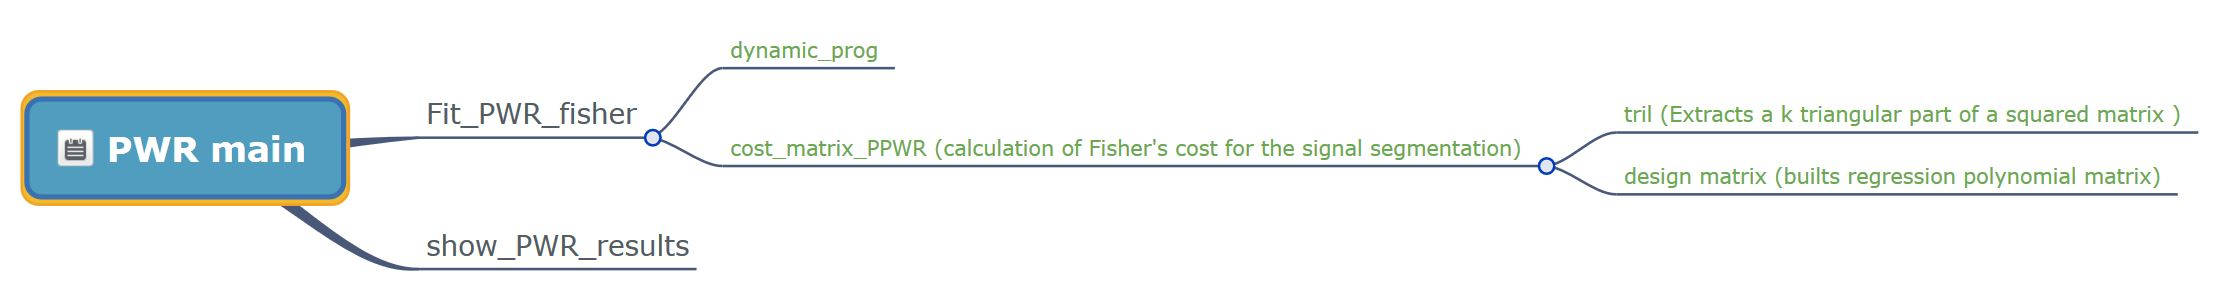
\includegraphics[scale=.6]{mindmapping.jpg}
\caption{\label{fig: mindmapping} Carte mentale de l'algorithme}
\end{figure} 
\smallbreak

\subsection{Description de la fonction : designmatrix }
\label{ssec: ssprog1}
\smallbreak
Cette fonction, permet, à partir d'un vecteur $\br_{i}$ et d'un degré de polynôme $p$, de construire la matrice de régression polynomiale de degré p $\bt$
$$
\bT=\begin{pmatrix}
   1 & \bt_{1} & \bt^2_{1} & \cdots & \bt^p_{1} \\
   1 & \bt_{2} & \bt^2_{2} & \cdots & \bt^p_{2}  \\
   \vdots & \vdots &\vdots &\vdots\\
   1 & \bt_{n} & \bt^2_{n} & \cdots & \bt^p_{n}  
\end{pmatrix}
$$

\smallbreak
\subsection{Description de la fonction : tril}
\label{ssec: ssprog2}
\smallbreak
Cette fonction a pour but de récupérer un k-triangule d'une matrice. k permet de déterminer à partir de quelle diagonale on fait l'extraction, et selon le signe de k, si on récupère les valeurs au dessus de cette kème diagonale ou en dessous.
Cette fonction existe dans Matlab, mais il a fallu la concevoir pour R.

\smallbreak
\subsection{Description de la fonction : cost-matrix-PPWR}
\label{ssec: ssprog3}
\smallbreak
Cette fonction a pour objectif de calculer la matrice coût de Fisher pour la segmentation du signal sur un intervalle $[a,b]$.
Elle est définie comme suit :
\begin{equation}
C(a,b) = \sum_{t=a}^{t=b}[ln(\sigma^2)+({\bx}_{t}-mu)^2/\sigma^2],
\label{eq:Eq5}
\end{equation}
avec mu = $\bsbeta^T \br_{t}$ : un polynôme d'ordre p. Ici $\bsbeta$ se calcule pour chaque couple (a,b).
  
  La fonction prend en entrée la variable d'intérêt de la série temporelle, le vecteur temps, l'ordre du polynôme de régression et Lmin : le nombre de  points minimum dans un segment (par défaut Lmin = 1) et ressort la matrice de coût, de dimension $n \times n$. La matrice de coût a au préalable été initialisée à l'infini.
   
Le code R a été amélioré par rapport à une limitation existant dans le code Matlab :une condition a été ajoutée sur la boucle de parcours de la matrice pour éviter d'en sortir.    
 \smallbreak
 
\subsection{Description de la fonction : dynamic-prog }
\label{ssec: ssprog4}
\smallbreak
Cette fonction réalise l'algorithme de programmation dynamique. Elle cherche la partition qui minimise le critère $ J(\bspsi,\bsgamma)$.
Elle prend comme entrée la matrice de coût sur l'intervalle $[a,b]$.
Cette fonction ressort le critère  $ J(\bspsi,\bsgamma)$ (vecteur de dimension $K \times 1$ contenant le critère pour chaque valeur du nombre d'intervalles k qui varie de 1 jusqu'à K et le temps de changement (partition) estimés (estimée) pour chaque valeur de k. C'est une matrice de dimension $Kmax \times Kmax$.

Une fois la partition estimée, les coefficients de régression associés à chaque segment ainsi que la variance du bruit sur chaque segment seront calculés par la méthode du maximum de vraisemblance dans la fonction suivante.

\smallbreak
\subsection{Description de la fonction : fit-PWR-fisher}
\label{ssec: ssprog5}
\smallbreak
Une fois la partition estimée par la fonction précédente : $"dynamic\_prog"$, cette fonction calcule les coefficients de régression associés à chaque segment ainsi que la variance du bruit sur chaque segment par la méthode du maximum de vraisemblance.
\smallbreak
\subsection{Description de la fonction : show-PWR-results}
\label{ssec: ssprog6}
\smallbreak
Cette fonction réalise la représentation graphique de la série initiale, de sa segmentation et des droites de régression pour chaque régime. Deux graphiques seront générés par le code, dans des fenêtres externes.
\smallbreak
\subsection{Description de la fonction : main-PWR-fisher}
\label{ssec: ssprog7}
\smallbreak
Cette dernière fonction (le programme principal) permet d'appeler les bibliothèques R nécessaires, définit les variables K et p, va récupérer le jeu de données et enfin source toutes les fonctions précédemment décrites pour faire tourner le programme. Ainsi 2 courbes s'affichent dans 2 fenêtres:

- la première (Fig\ref{fig: segmentation1}) présente la série temporelle initiale, et les polynômes qui l'approchent pour chaque régime. Chacune des courbes des polynômes a sa propre couleur, et la partie correspondant au régime associé est présentée en trait plus épais (en pointillé pour le reste).
- la seconde  (Fig\ref{fig: segmentation2}) représente la série temporelle initiale, et la segmentation optimale avec en rouge la courbe de régression pour chaque régime.  

Les figures ci-dessous présentent les sorties du code R pour un exemple de série temporelle.
\smallbreak
\begin{figure}[H] 
\centering
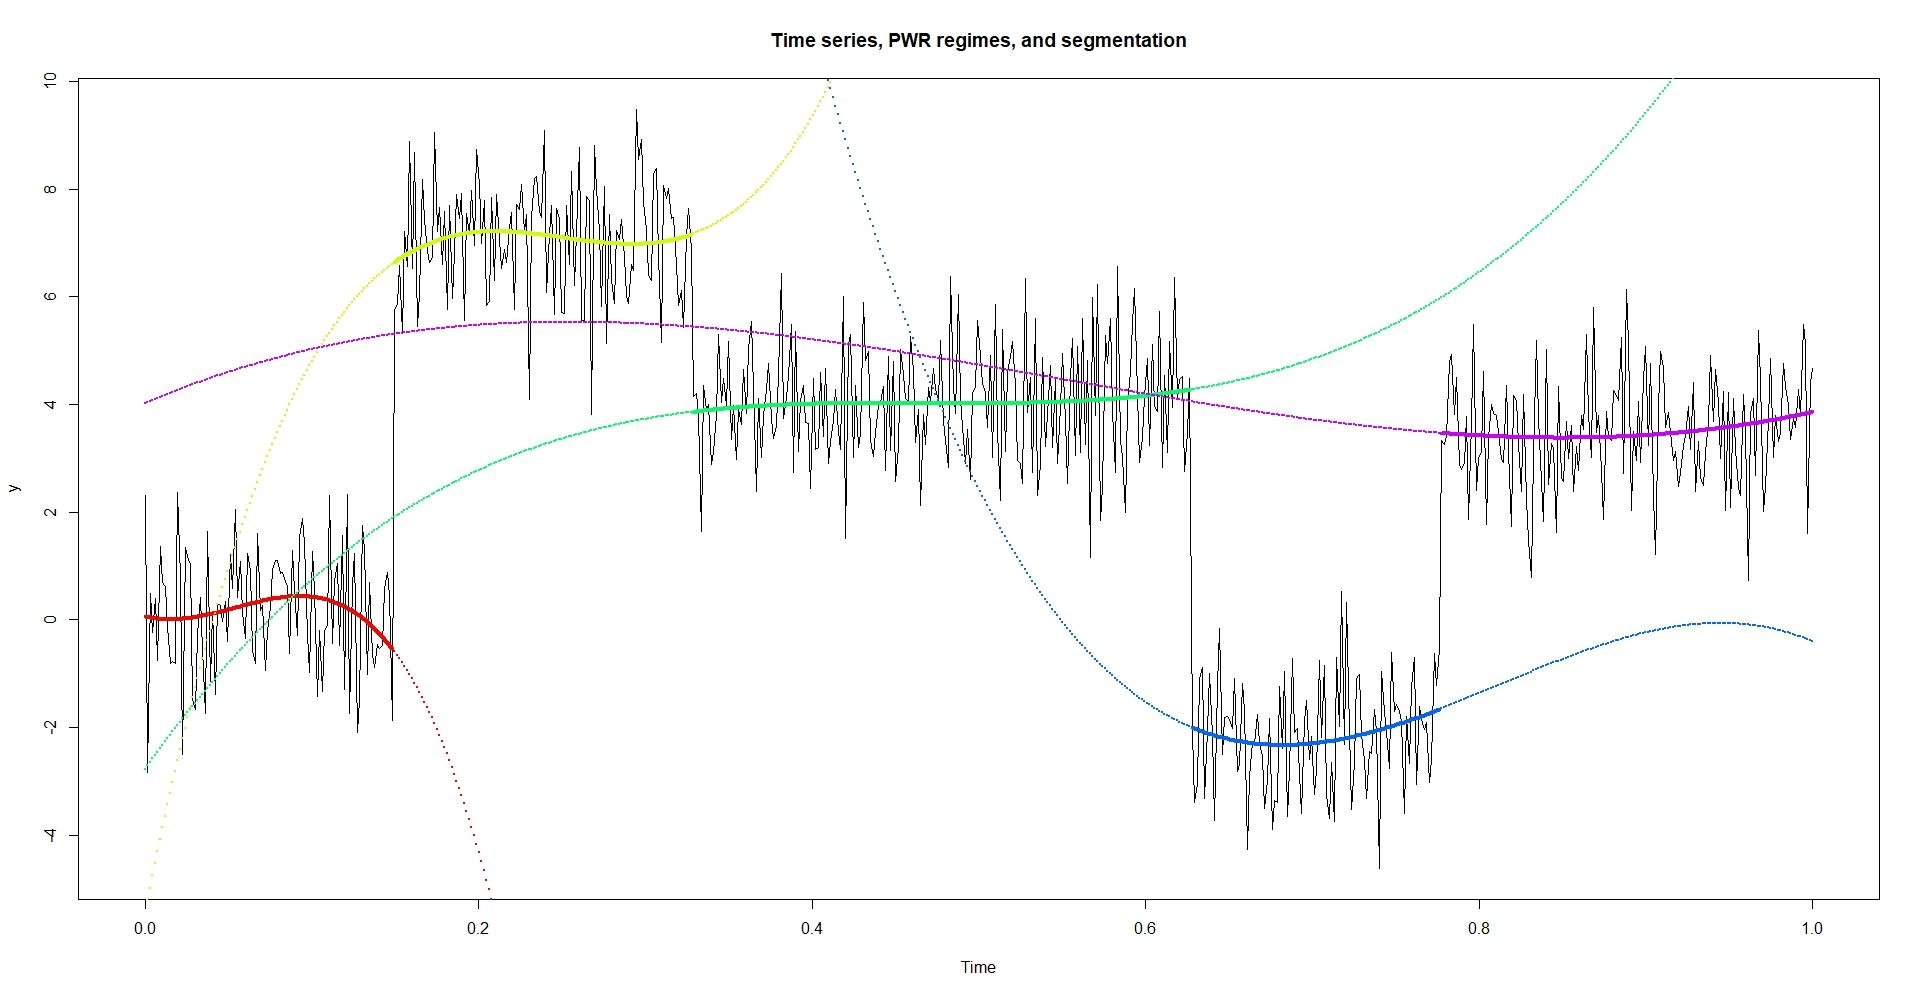
\includegraphics[scale=.25]{segmentation1.jpeg}
\caption{\label{fig: segmentation1} Série temporelle et fonctions de régressions polynomiales}
\end{figure}

\begin{figure}[H] 
\centering
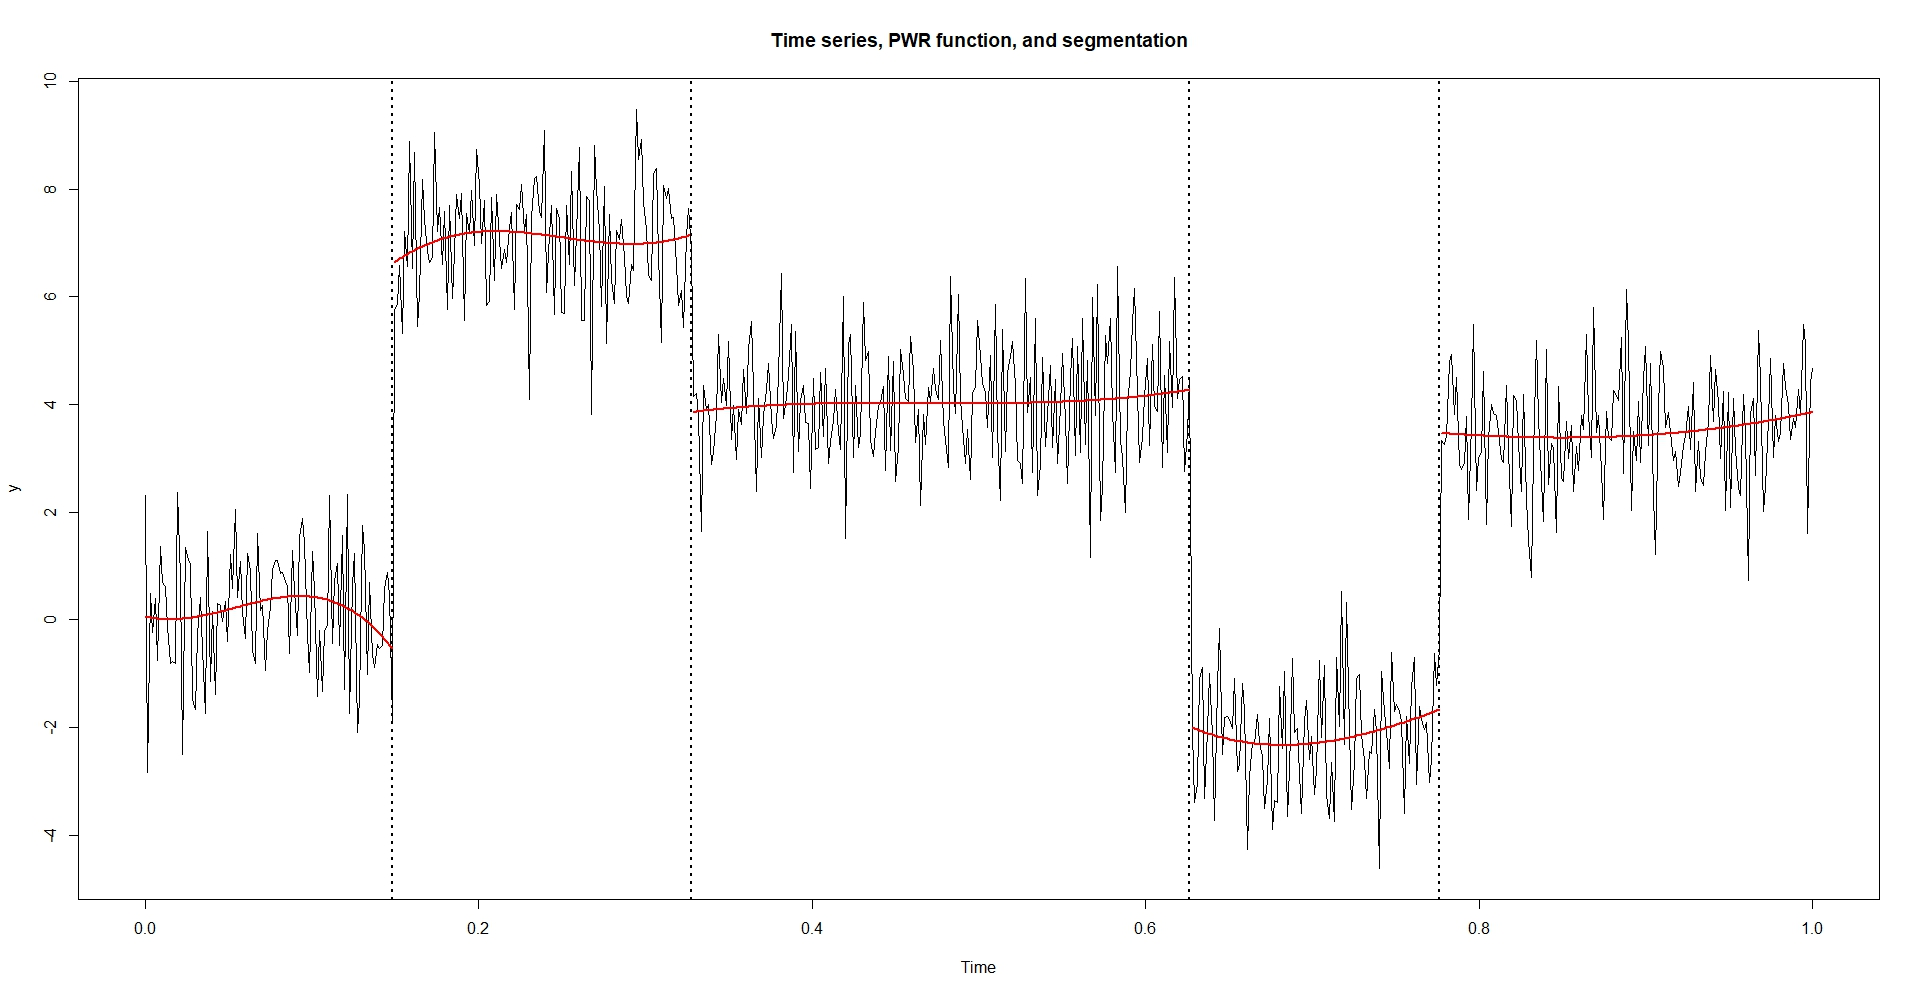
\includegraphics[scale=.25]{segmentation.jpeg}
\caption{\label{fig: segmentation2} Série temporelle segmentée et approximée par les régressions polynomiales}
\end{figure} 


\section{Conclusion}
\label{sec:Conclusion}
Cette méthode de segmentation a donc permis de retrouver les différents régimes de la série temporelle et les coefficients de régression pour chaque région. Elle peut fonctionner pour n'importe quel degré de polynôme à partir de $p=0$. Par rapport au code Matlab, il a fallu rajouter une fonction d'extraction d'un triangle dans une matrice (qui n'existe pas en R), et séparer le cas p=0 car R considère qu'une matrice de dimension 1 est un vecteur et ne permet pas de faire des calculs matriciels. En terme de vitesse d'exécution des programmes, Matlab est plus de 3 fois plus rapide, avec 8.63 secondes contres 29.1 secondes sous R. Enfin, les représentations graphiques et les résultats calculatoires des 2 programmes (R et Matlab) sont exactement les mêmes.


\newpage
\bibliographystyle{alpha}
\bibliography{REFERENCES}

\end{document}
